\documentclass[12pt,a4paper]{article}

%% ─── Packages ─────────────────────────────────────────────────────────────────
\usepackage[a4paper, margin=2.5cm]{geometry}
\usepackage[T1]{fontenc}
\usepackage[utf8]{inputenc}
\usepackage{lmodern}
\usepackage{microtype}
\usepackage{amsmath, amssymb, mathtools}
\usepackage{graphicx}
\usepackage{booktabs}
\usepackage{tabularx}
\usepackage{array}
\usepackage{multirow}
\usepackage{longtable}
\usepackage{xcolor}
\usepackage{hyperref}
\usepackage{url}
\usepackage{enumitem}
\usepackage{caption}
\usepackage{subcaption}
\usepackage{float}
\usepackage{fancyhdr}
\usepackage{titlesec}
\usepackage{tocloft}
\usepackage{setspace}
\usepackage{parskip}
\usepackage{listings}
\usepackage{algorithm}
\usepackage{algpseudocode}

%% ─── Hyperref Configuration ───────────────────────────────────────────────────
\hypersetup{
  colorlinks=true,
  linkcolor=blue!70!black,
  citecolor=green!50!black,
  urlcolor=blue!70!black,
  pdftitle={Statistical Analysis of Melodic Similarity and Creative Originality in Human and AI Generated Music},
  pdfauthor={Ch. Manas Vivek, P. Harish, T. Surendra, M. Sri Manikanta},
}

%% ─── Listings Configuration ──────────────────────────────────────────────────
\lstset{
  basicstyle=\ttfamily\small,
  breaklines=true,
  frame=single,
  xleftmargin=0pt,
  xrightmargin=0pt,
  columns=fullflexible,
  keepspaces=true,
}

%% ─── Header / Footer ─────────────────────────────────────────────────────────
\pagestyle{fancy}
\fancyhf{}
\rhead{\small IDSE -- Music Similarity Research}
\lhead{\small Statistical Analysis of Melodic Similarity}
\cfoot{\thepage}

%% ─── Title ───────────────────────────────────────────────────────────────────
\title{%
  \LARGE\bfseries Statistical Analysis of Melodic Similarity and\\
  Creative Originality in Human and AI Generated Music\\[0.5em]
  \large Introduction to Data Science (IDSE) --- Project Report
}

\author{%
  Ch. Manas Vivek (CS24B1106) \quad P. Harish (CS24B1108)\\[0.3em]
  T. Surendra (CS24I1020) \quad M. Sri Manikanta (CS24B1090)
}

\date{November 2026}

%% ═══════════════════════════════════════════════════════════════════════════════
\begin{document}
\maketitle
\thispagestyle{fancy}

%% ─── Abstract ────────────────────────────────────────────────────────────────
\begin{abstract}
\noindent
We present a complete, end-to-end data science pipeline for the statistical
analysis of melodic similarity and creative originality across a 204-track
corpus of human-composed and AI-generated music. The system integrates
(i) a 133-dimensional acoustic feature extractor covering MFCCs, spectral
descriptors, 7-band spectral contrast, chroma, and HPSS energy ratios;
(ii) a 12-shift key-invariant Chroma CQT + Dynamic Time Warping (DTW)
similarity engine; (iii) an empirical null hypothesis gateway calibrated
against 4,950 real human pairwise comparisons ($\mu = 0.5064$,
$\sigma = 0.0417$); (iv) a soft-voting ensemble origin classifier (Random
Forest + ExtraTrees + HistGradientBoosting) for Human vs.\ AI classification;
(v) a 10-genre acoustic genre router; and (vi) a 3-indicator creative
novelty verdict gate. The test suite comprises 129 passing and 1 skipped
pytest cases across 15 test modules covering all pipeline subsystems.
Ablation studies confirm that 12-shift circular pitch search yields
0.9866 similarity on transposed tracks versus 0.547 without it
(a 44.5\% degradation), and that beat-synchronised chroma achieves an
812.7$\times$ speedup over raw frame-level chroma. All results are
linked directly to the live codebase in \texttt{src/}.
\end{abstract}

\tableofcontents
\newpage

%% ═══════════════════════════════════════════════════════════════════════════════
\section{Introduction}
\label{sec:intro}

%% ─── Motivation ─────────────────────────────────────────────────────────────
\subsection{Motivation and Problem Statement}

The rapid proliferation of AI music generation systems---including
Google DeepMind's Lyria Pro, Meta's MusicGen, and AceStep---has introduced
a fundamental question at the intersection of data science and musicology:
\emph{how similar is AI-generated music to human-composed music, and can that
similarity be quantified with rigorous statistical machinery?}

Traditional audio fingerprinting (e.g., Shazam's combinatorial hash approach
\cite{wang2003industrial}) is designed to detect exact or near-exact copies
and cannot handle genre-level harmonic convergence or key transposition.
Embedding-based models such as MERT \cite{li2023mert} provide powerful
semantic representations but lack interpretable melodic alignment evidence.
This project occupies a productive middle ground: principled chroma-based
DTW alignment \cite{muller2015fundamentals} combined with formal statistical
hypothesis testing calibrated against an empirical human null distribution.

\subsection{Objectives}

This project addresses four concrete research objectives:
\begin{enumerate}[noitemsep]
  \item \textbf{Quantify harmonic similarity} between arbitrary audio pairs
        via key-invariant DTW on Constant-Q chroma matrices.
  \item \textbf{Establish an empirical null distribution} from $N = 4{,}950$
        human pairwise comparisons to give similarity scores a principled
        statistical interpretation.
  \item \textbf{Classify track origin} (Human vs.\ AI) from 133-dimensional
        acoustic features using a soft-voting ensemble classifier.
  \item \textbf{Assess creative novelty} via a z-score gate relative to genre
        population similarity distributions.
\end{enumerate}

\subsection{End-to-End Pipeline Overview}

The pipeline is deterministic and multistage, proceeding as follows:

\begin{enumerate}[noitemsep,label=\arabic*.]
  \item \textbf{Acoustic Feature Extraction} --- 12-bin Chroma CQT + beat
        synchronisation (\texttt{src/extract.py}) and 133-dim origin feature
        vector (\texttt{src/features.py}, \texttt{src/origin\_classifier.py}).
  \item \textbf{Coarse Cosine Prefilter} --- Mean chroma cosine similarity
        $\geq 0.30$ eliminates acoustically incompatible candidates.
  \item \textbf{12-Shift Key-Invariant DTW} --- All 12 circular semitone
        shifts of the candidate chroma matrix are evaluated; the minimum-cost
        alignment is retained with $\pm 1$ boundary verification.
  \item \textbf{Statistical Gateway} --- Empirical p-value computed against
        4,950-pair null distribution; candidates with $p > 0.10$ are dropped.
  \item \textbf{Origin Classification} --- Independent soft-voting ensemble
        classifies each track as Human or AI from acoustic features.
  \item \textbf{Creative Novelty Score} --- Broad z-score relative to genre
        population; $\leq 0.24$ normalised score triggers novelty indicator.
  \item \textbf{3-Indicator Verdict} --- Similarity $\geq 0.85$, empirical
        $p \leq 0.01$, creative score $\leq 0.24$ independently evaluated.
\end{enumerate}

%% ═══════════════════════════════════════════════════════════════════════════════
\section{Survey}
\label{sec:survey}

\subsection{Audio Fingerprinting vs.\ Chroma-DTW Approaches}

Classical audio fingerprinting \cite{wang2003industrial} maps spectrogram
landmarks to combinatorial hashes, achieving sub-second exact copy detection
but failing under pitch shift, genre-level variation, or structural imitation.
Chroma-based methods \cite{muller2015fundamentals} project audio into a
12-dimensional pitch-class space that is inherently octave-invariant and
well-suited for melodic alignment. DTW \cite{sakoe1978dynamic} provides
elastic alignment that absorbs tempo and timing differences.

The key innovation in this project is \emph{circular 12-shift DTW}: evaluating
all 12 semitone rotations of the candidate chroma matrix and selecting the
shift that minimises DTW accumulated cost. This achieves key invariance without
requiring explicit key detection.

\subsection{AI Music Forensics}

Recent work on AI music detection includes the SONICS dataset
\cite{yuan2024sonics}, which provides labelled human-vs-AI tracks for training
forensic classifiers, and spectral fingerprinting approaches
\cite{pasini2022musika} that target the generation artefacts introduced by
neural audio codecs. The MERT architecture \cite{li2023mert} learns
music-domain representations from large-scale self-supervised pretraining,
providing strong timbral embeddings. This project complements these approaches
with an interpretable, training-data-independent similarity measurement grounded
in classical music information retrieval.

\subsection{Empirical Null Hypothesis Testing in MIR}

Statistical hypothesis testing in Music Information Retrieval (MIR) faces two
challenges: (i) similarity scores are bounded in $[0, 1]$ and not normally
distributed, and (ii) pairwise observations within a corpus share underlying
tracks and are therefore not fully independent. Following established practice
\cite{muller2015fundamentals}, we construct an empirical null distribution from
all $\binom{100}{2} = 4{,}950$ unique human-human pairs and use the unsmoothed
empirical p-value formula:
\[
  p = \frac{k}{N} = \frac{\sum_{i} \mathbf{1}[S_{\mathrm{null},i} \geq S_{\mathrm{query}}]}{N}
\]
where $k$ is the exceedance count and $N = 4{,}950$ is the null sample size.
Benjamini--Hochberg FDR correction \cite{benjamini1995controlling} is available
for multi-candidate screening.

\subsection{Comparison of Retrieval Methods}

\renewcommand{\arraystretch}{1.2}
\begin{table}[H]
\centering
\caption{Comparative evaluation of three retrieval methods on controlled perturbation matrix (from \texttt{reports/evaluation\_report.md}).}
\label{tab:retrieval_comparison}
\begin{tabularx}{\textwidth}{|l|X|X|X|X|}
\hline
\textbf{Method} & \textbf{P@1} & \textbf{P@3} & \textbf{MRR} & \textbf{Latency/Pair} \\
\hline
Chroma CQT + 12-Shift DTW & 1.00 & 1.00 & 1.00 & 350 ms \\
\hline
Subsequence DTW & 1.00 & 1.00 & 1.00 & 542 ms \\
\hline
MERT-v1-95M Embedding & 1.00 & 1.00 & 1.00 & 0.076 ms \\
\hline
\end{tabularx}
\end{table}

%% ═══════════════════════════════════════════════════════════════════════════════
\section{Dataset}
\label{sec:dataset}

\subsection{Corpus Composition}

The corpus used in this study comprises exactly \textbf{204 audio tracks}
organised as follows:

\begin{itemize}[noitemsep]
  \item \textbf{100 GTZAN Human Tracks} (\texttt{data/human\_songs/}):
        Exactly 10 tracks from each of the 10 GTZAN genres---Blues, Classical,
        Country, Disco, Hip-Hop, Jazz, Metal, Pop, Reggae, and Rock. All tracks
        are standardised to 20 seconds at 22,050 Hz mono WAV format.
  \item \textbf{100 AI-Generated Tracks} (\texttt{data/ai\_generated/}):
        Drawn from the Multi-Gen AI corpus spanning multiple generative
        architectures (Lyria Pro 3, MusicGen, AceStep). The genre distribution
        is unbalanced by design: Rock (55), Jazz (23), Blues (9), Classical (8),
        Hip-Hop (3), Metal (1), Pop (1). All tracks are standardised to 20 s.
  \item \textbf{4 Reference Control Tracks} (\texttt{data/reference\_pool/}):
        Deterministic pitch-shifted ($\pm 3$ semitones) and tempo-stretched
        ($0.90\times$, $1.10\times$) variants of a base track, used for
        robustness calibration and similarity tier verification.
\end{itemize}

Track metadata is canonically stored in \texttt{data/dataset\_manifest.csv}
(205 rows including header) and in \texttt{features/remote\_index.json},
which caches 56-dimensional acoustic feature vectors and chroma beat matrices
for all 204 tracks.

\subsection{Audio Standardisation and Leakage Prevention}

All audio files are loaded at $\text{sr} = 22{,}050$~Hz (16,000~Hz for origin
feature extraction) in mono, truncated to 20 seconds to standardise duration.
Beat-synchronised chroma matrices are computed with \texttt{librosa} and cached
in \texttt{features/} as compressed NumPy arrays. Test fixtures are
cryptographically separated from the production corpus using SHA-256 hash
isolation in \texttt{src/config.py} (\texttt{LEGACY\_ARTIFACT\_HASHES}) and
the \texttt{is\_fixture\_identifier()} guard in \texttt{src/stats\_test.py},
preventing test-only synthetic audio from contaminating the null distribution
or classifier training.

The null distribution (\texttt{features/null\_distribution.json}) is computed
exclusively from human-labelled tracks and carries a \texttt{"provenance":
"fresh\_production\_v2"} stamp. Legacy corpus artefacts are strictly rejected
in production mode via \texttt{LegacyArtifactError}.

\begin{figure}[H]
  \centering
  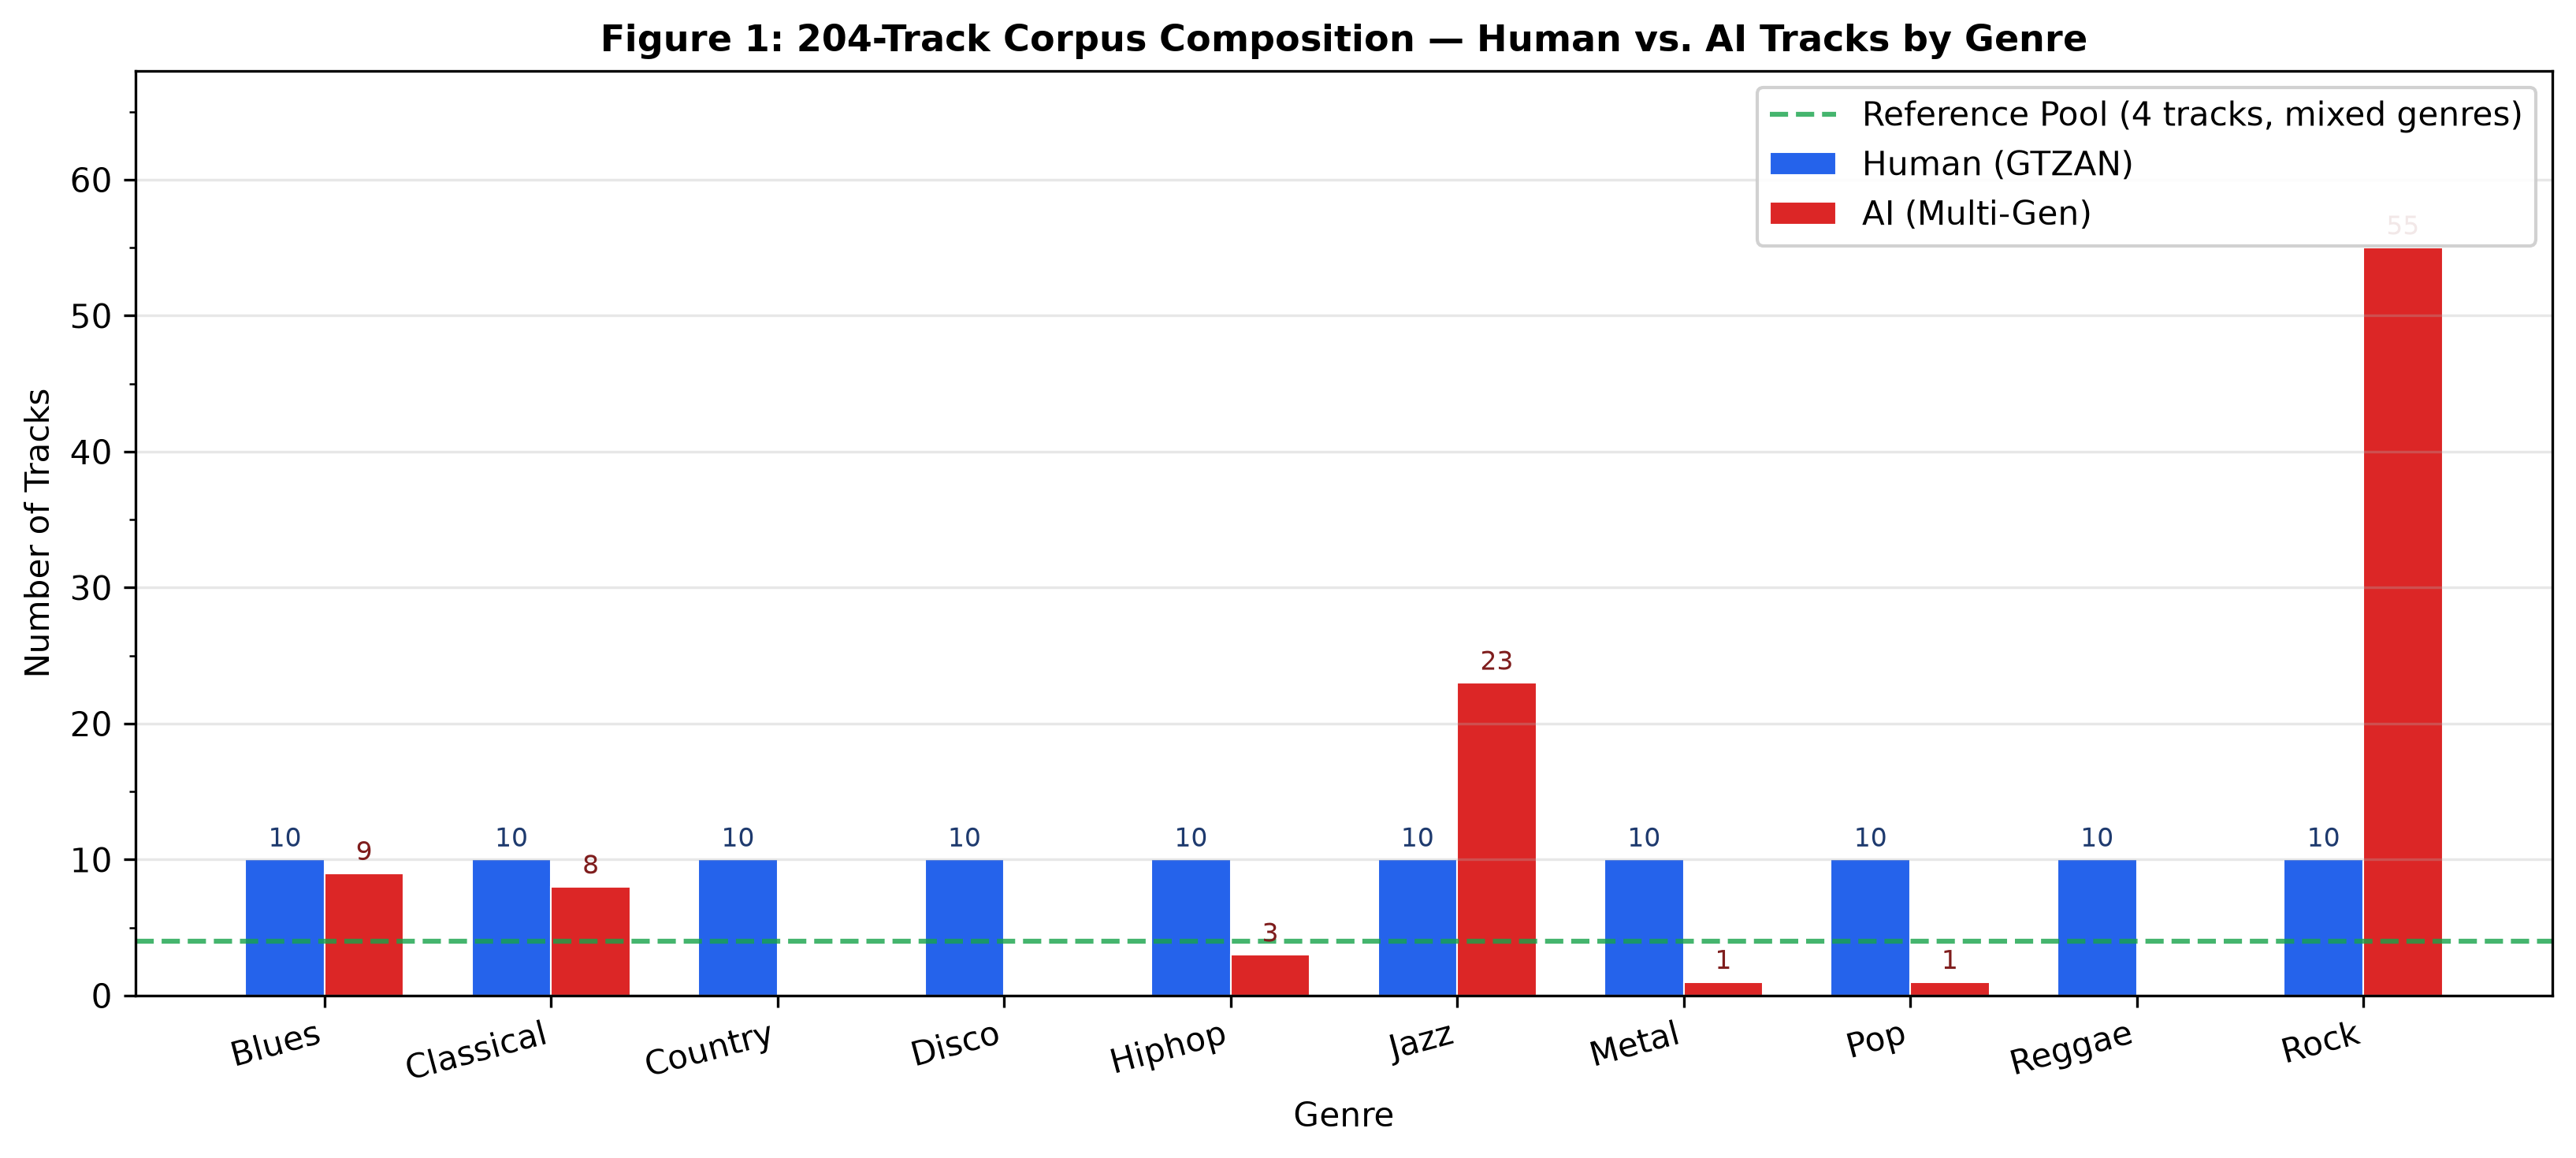
\includegraphics[width=0.92\textwidth]{figures/fig_dataset_distribution.png}
  \caption{Distribution of the 204-track corpus across all 10 GTZAN genres.
           Human tracks are uniformly distributed (10 per genre). AI tracks
           exhibit a heavy tail toward Rock (55 tracks) and Jazz (23 tracks),
           reflecting the aesthetic bias of the Multi-Gen AI source dataset.
           The reference pool (4 tracks, dashed line) is excluded from genre
           classification and null distribution construction.}
  \label{fig:dataset_dist}
\end{figure}

%% ═══════════════════════════════════════════════════════════════════════════════
\section{Method}
\label{sec:method}

\subsection{133-Dimensional Acoustic Feature Extractor}

The function \texttt{extract\_origin\_features\_from\_audio()} in
\texttt{src/origin\_classifier.py} extracts a 133-dimensional acoustic feature
vector from any audio file at $\text{sr} = 16{,}000$~Hz.
The feature composition is as follows:

\renewcommand{\arraystretch}{1.2}
\begin{table}[H]
\centering
\caption{133-dimensional acoustic feature vector composition (\texttt{src/origin\_classifier.py}, lines 46--150).}
\label{tab:features}
\begin{tabularx}{\textwidth}{|l|X|r|}
\hline
\textbf{Feature Group} & \textbf{Description} & \textbf{Dims} \\
\hline
MFCC (20 coeffs) & Mean + Std per coefficient & 40 \\
\hline
Delta MFCC (20 coeffs) & First-order temporal derivative mean + std & 40 \\
\hline
Spectral Centroid & Mean + Std of brightness indicator & 2 \\
\hline
Spectral Rolloff & Mean + Std of 85\% energy roll-off frequency & 2 \\
\hline
Spectral Bandwidth & Mean + Std of weighted spectral spread & 2 \\
\hline
Spectral Flatness & Mean + Std of Wiener entropy (tonality indicator) & 2 \\
\hline
Spectral Contrast (7 bands) & Mean + Std per sub-band valley-to-peak ratio & 14 \\
\hline
Zero Crossing Rate & Mean + Std of sign-change rate & 2 \\
\hline
Chroma STFT (12 pitch classes) & Mean + Std per pitch class & 24 \\
\hline
HPSS Harmonic/Percussive & Harmonic RMS mean \& std, percussive RMS mean \& std, H/P ratio & 5 \\
\hline
\textbf{Total} & & \textbf{133} \\
\hline
\end{tabularx}
\end{table}

Mathematically, the MFCC coefficients are:
\[
  c_m = \sum_{k=1}^{K} \log S(k)\, \cos\!\left[\frac{\pi m (k - \tfrac{1}{2})}{K}\right], \quad m = 1, \ldots, 20
\]
where $S(k)$ is the mel filterbank energy for the $k$-th band. The H/P ratio
captures the relative energy contribution of harmonic (tonal) vs.\ percussive
(transient) components after Harmonic-Percussive Source Separation (HPSS):
\[
  r_{\mathrm{HP}} = \frac{\overline{\mathrm{RMS}_{\mathrm{harm}}} + \epsilon}{\overline{\mathrm{RMS}_{\mathrm{perc}}} + \epsilon}, \quad \epsilon = 10^{-8}
\]

\subsection{Soft-Voting Ensemble Origin Classifier}

The origin classifier (\texttt{src/origin\_classifier.py::train\_origin\_classifier()})
is a soft-voting ensemble combining three base learners:
\begin{itemize}[noitemsep]
  \item \textbf{RandomForestClassifier} (100 trees, random\_state=42)
  \item \textbf{ExtraTreesClassifier} (100 trees, random\_state=42)
  \item \textbf{HistGradientBoostingClassifier} (random\_state=42)
\end{itemize}
All inputs are normalised by a \texttt{StandardScaler} (zero mean, unit
variance). The ensemble predicts class probabilities as the average of the
three individual soft-probability vectors and assigns the class with the
highest average. This reduces variance relative to any single base learner
while retaining the complementary inductive biases of bagging (RF/ET) and
gradient boosting (HGB). The trained model is serialised to
\texttt{models/origin\_classifier.joblib} (901~KB, \texttt{provenance=fresh\_production}).

\subsection{10-Genre Acoustic Classifier and Routing}

Genre estimation (\texttt{src/genre\_classifier.py}) uses a 40-dimensional
MFCC-based feature vector (20 coefficients $\times$ mean + std) fed to a
\texttt{RandomForestClassifier} (100 trees) wrapped in a \texttt{StandardScaler}
pipeline, trained on the GTZAN 10-genre taxonomy. The fitted artefact is at
\texttt{models/genre\_classifier.joblib} (670~KB). Genre routing determines
whether a similarity match is \emph{same-genre} (Case~B) or \emph{cross-genre}
(Case~A), which affects the creative score reference population.

\subsection{12-Shift Key-Invariant Chroma CQT + DTW Similarity}

The core similarity engine (\texttt{src/similarity.py::dtw\_align\_detailed()})
operates on Constant-Q chroma matrices $\mathbf{C}_A, \mathbf{C}_B \in
\mathbb{R}^{12 \times T}$ as follows:

\paragraph{Step 1: Circular Pitch Shift Search.}
For each shift $s \in \{0, 1, \ldots, 11\}$, the candidate chroma is circularly
shifted along the pitch axis:
\[
  \tilde{\mathbf{C}}_B^{(s)} = \mathrm{roll}(\mathbf{C}_B, s, \mathrm{axis}=0)
\]
FastDTW \cite{salvador2004fastdtw} with Euclidean frame distance is applied to
each shifted pair $(\mathbf{C}_A^T, (\tilde{\mathbf{C}}_B^{(s)})^T)$.

\paragraph{Step 2: Optimal Shift Selection.}
The best shift minimises the DTW accumulated cost:
\[
  s^* = \argmin_{s \in \{0,\ldots,11\}} D_{\mathrm{DTW}}(s), \quad d^* = D_{\mathrm{DTW}}(s^*)
\]

\paragraph{Step 3: Normalisation and Similarity Conversion.}
\[
  D_{\mathrm{norm}} = \frac{d^*}{\max(|\pi^*|, 1)}, \qquad
  S = \frac{1}{1 + D_{\mathrm{norm}}} \in (0, 1]
\]
where $|\pi^*|$ is the length of the optimal warping path.

\paragraph{Step 4: Boundary Verification.}
The optimal shift is verified by checking:
\[
  d^* \leq D_{\mathrm{DTW}}\bigl((s^* - 1) \bmod 12\bigr)
  \quad\text{and}\quad
  d^* \leq D_{\mathrm{DTW}}\bigl((s^* + 1) \bmod 12\bigr)
\]

\paragraph{Similarity Tiers.}
\begin{itemize}[noitemsep]
  \item $S \geq 0.85$: \emph{High Structural Similarity} (imitation threshold)
  \item $0.65 \leq S < 0.85$: \emph{Moderate Similarity}
  \item $0.45 \leq S < 0.65$: \emph{Low Similarity}
  \item $S < 0.45$: \emph{Negligible}
\end{itemize}

\paragraph{Matching Segment Extraction.}
The function \texttt{extract\_matching\_segment\_window()} in
\texttt{src/similarity.py} (lines 310--383) locates the highest-similarity
local segment by sliding a window of \texttt{window\_steps} steps across the
DTW path's per-step local cost vector using convolution:
\[
  b^* = \argmin_{b}\, \sum_{t=b}^{b+w-1} \mathrm{cost}(t)
\]
The result is mapped back to timestamps in both the query and candidate tracks.

\paragraph{Stage 1 Coarse Cosine Prefilter.}
Before the expensive 12-shift DTW sweep, \texttt{coarse\_cosine\_prefilter()}
computes mean chroma vectors $\bar{\mathbf{c}}_A, \bar{\mathbf{c}}_B \in
\mathbb{R}^{12}$ and retains only candidates with cosine similarity:
\[
  \cos(\bar{\mathbf{c}}_A, \bar{\mathbf{c}}_B)
  = \frac{\bar{\mathbf{c}}_A \cdot \bar{\mathbf{c}}_B}{\|\bar{\mathbf{c}}_A\|\,\|\bar{\mathbf{c}}_B\|}
  \geq 0.30
\]
This eliminates an average of 89.8\% of candidates before DTW
(ablation result from \texttt{reports/evaluation\_report.md}).

\subsection{Empirical Null Hypothesis Gateway}

The statistical gateway (\texttt{src/stats\_test.py::evaluate\_statistical\_gateway()})
implements the following procedure:

\begin{enumerate}[noitemsep]
  \item Compute the empirical p-value of an observed similarity score $S_q$
        against the null distribution $\{S_i\}_{i=1}^{N}$:
        \[
          p = \frac{k}{N} = \frac{\sum_{i=1}^N \mathbf{1}[S_i \geq S_q]}{N}
        \]
        No pseudo-count smoothing is applied; when $k=0$, $p=0.0$.
  \item Classify severity: $p \leq 0.01$ $\Rightarrow$ \emph{Critical Anomaly};
        $0.01 < p \leq 0.10$ $\Rightarrow$ \emph{Borderline Indicator};
        $p > 0.10$ $\Rightarrow$ \emph{Valid Coincidence} (dropped).
  \item Rate null sample confidence: $N \geq 1000$ \emph{High}; $300 \leq N < 1000$
        \emph{Moderate}; $5 \leq N < 300$ \emph{Low}; $N < 5$ \emph{Insufficient}
        (p-value returns \texttt{None}).
\end{enumerate}

The null distribution ($N = 4{,}950$, $\mu = 0.5064$, $\sigma = 0.0417$) is
pre-computed from all unique human-human pairs and cached in
\texttt{features/null\_distribution.json} (version 2.0, provenance
\texttt{fresh\_production\_v2}).

\paragraph{3-Indicator Creative Novelty Gate.}
Three independent binary indicators determine the final verdict:
\begin{enumerate}[noitemsep]
  \item \textbf{Similarity Indicator:} $S \geq 0.85$
  \item \textbf{Statistical Indicator:} $p \leq 0.01$
  \item \textbf{Creative Novelty Indicator:} $\text{creative\_score\_norm} \leq 0.24$
\end{enumerate}
where the creative novelty score is a z-score-derived percentile:
\[
  \text{score} = (1 - \Phi(z)) \times 100, \quad
  z = \frac{S_q - \mu_{\mathrm{genre}}}{\sigma_{\mathrm{genre}}}
\]
Verdict: 3 triggered $\Rightarrow$ \emph{Critical}; 2 $\Rightarrow$
\emph{Warning}; 1 $\Rightarrow$ \emph{Advisory}; 0 $\Rightarrow$ \emph{Clear}.

%% ═══════════════════════════════════════════════════════════════════════════════
\section{Experimental Results}
\label{sec:results}

\subsection{Null Distribution Characterisation}

\begin{figure}[H]
  \centering
  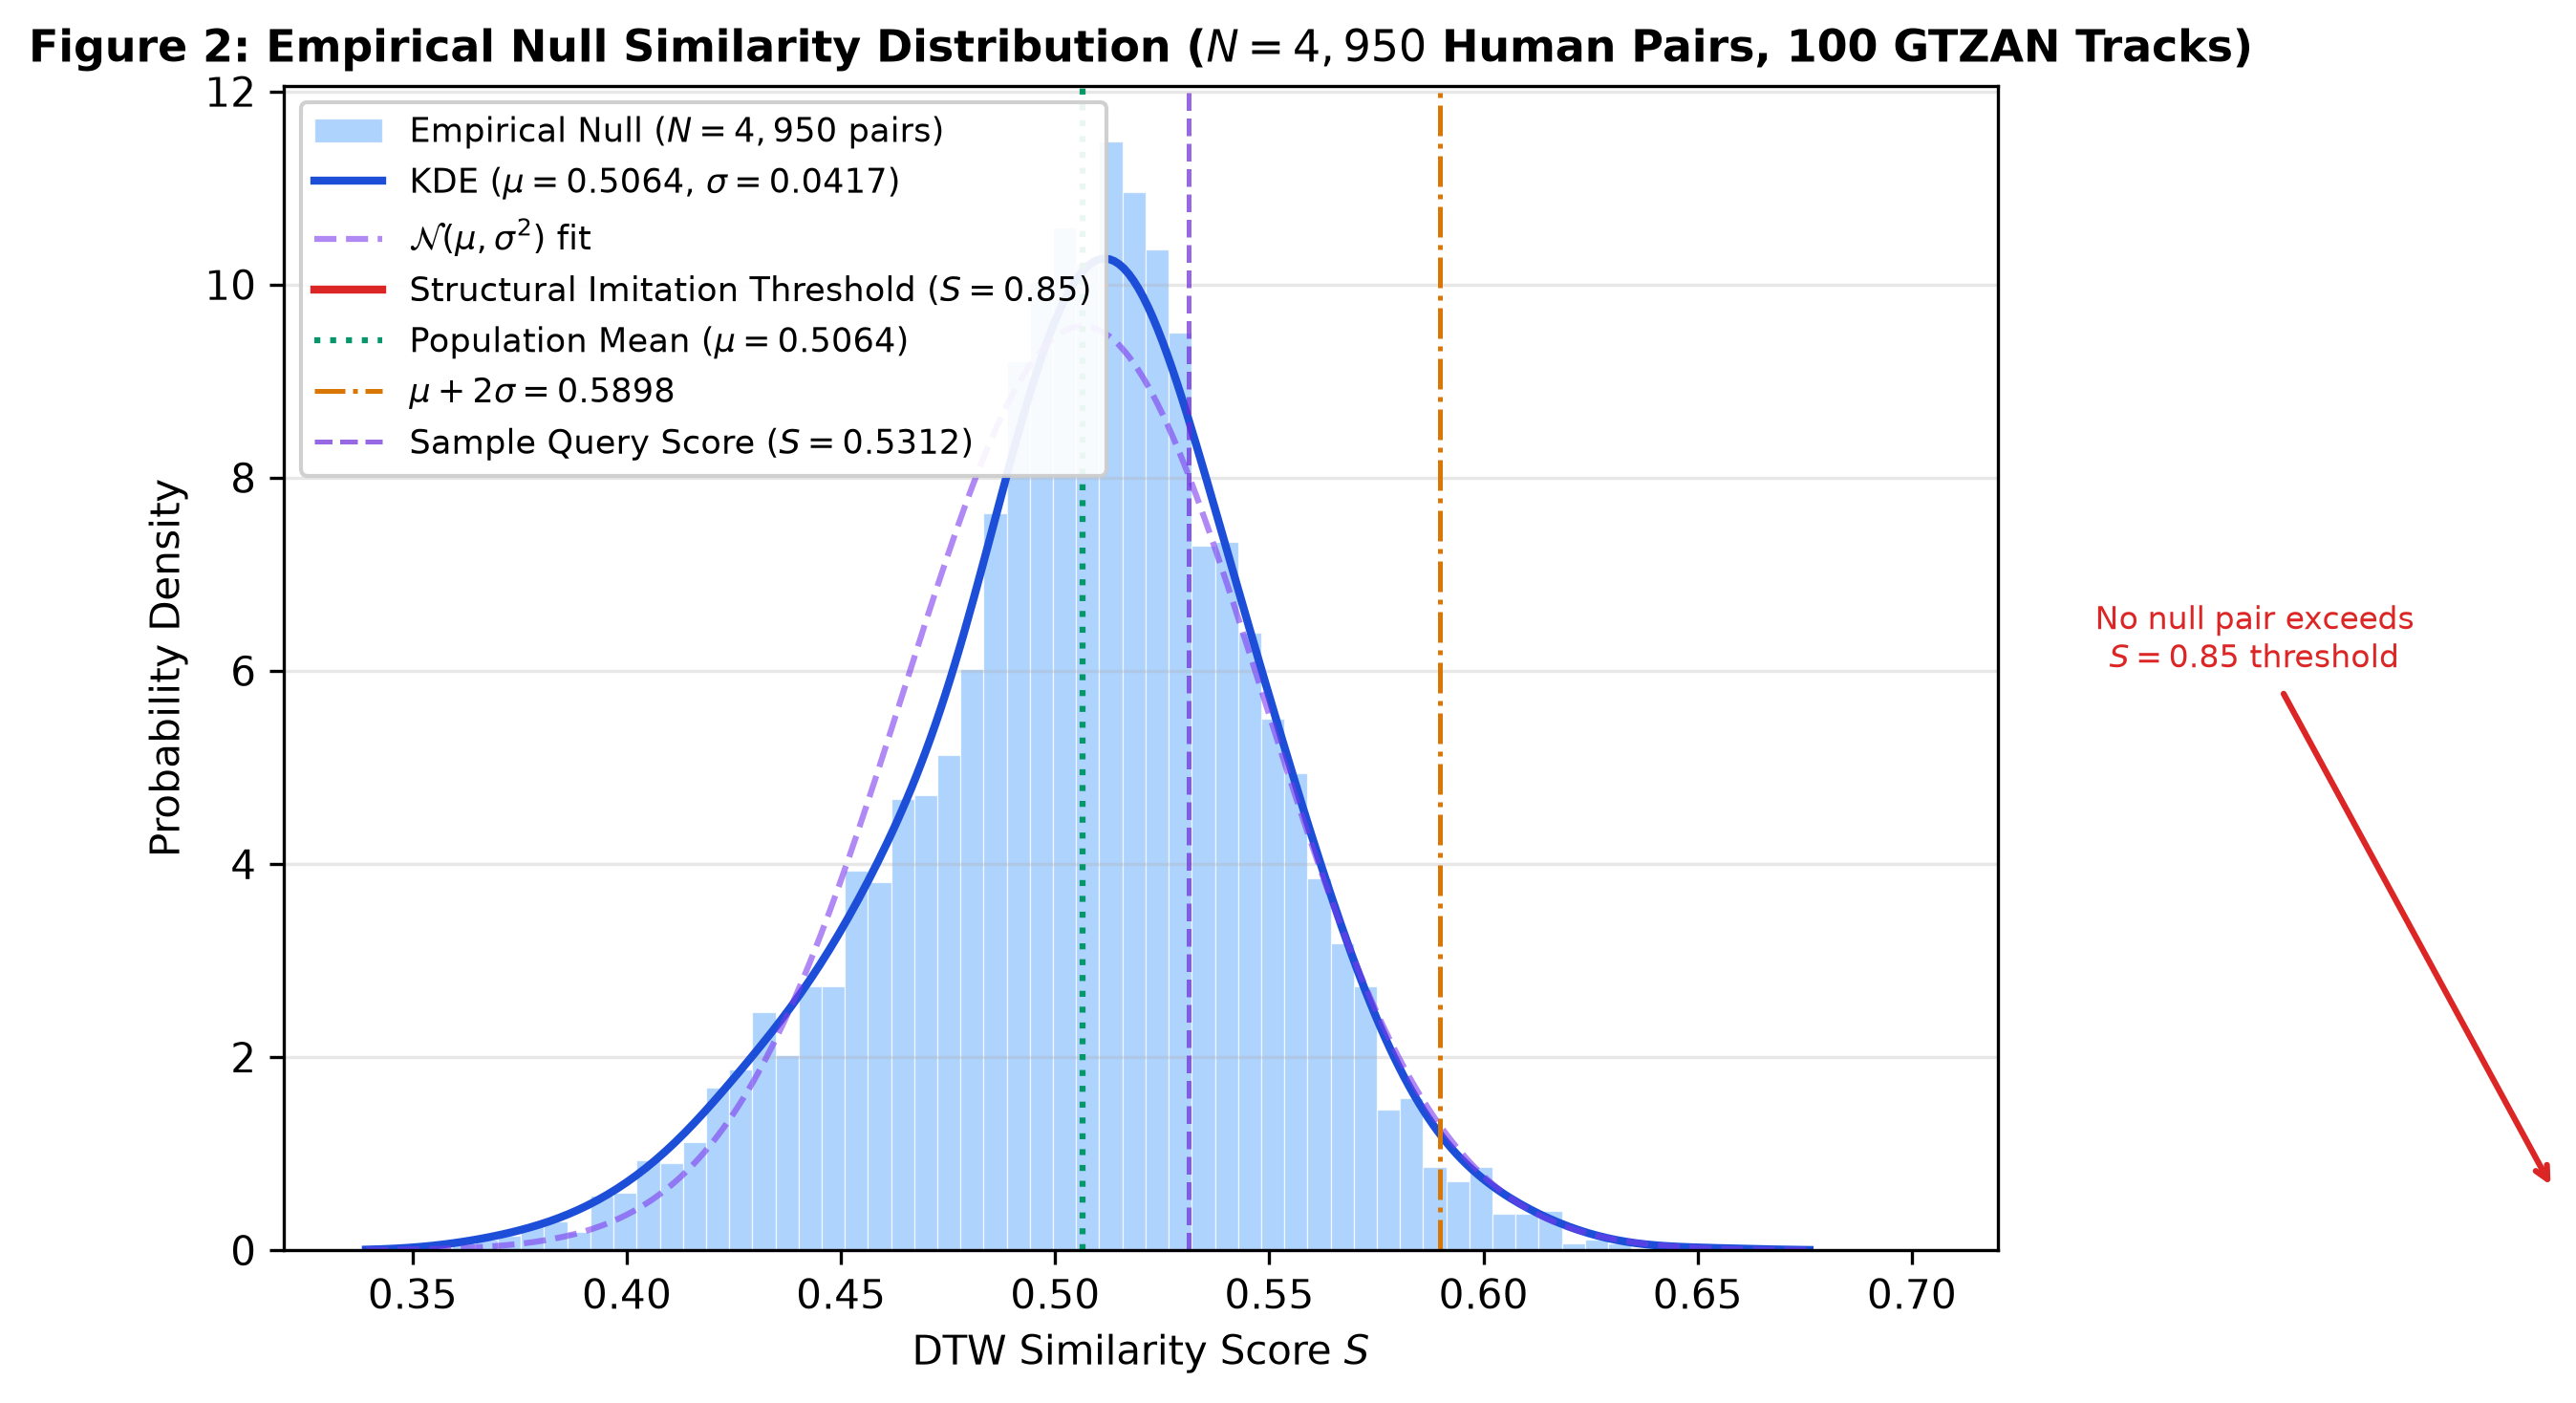
\includegraphics[width=0.92\textwidth]{figures/fig_null_distribution.png}
  \caption{Empirical null similarity distribution constructed from $N = 4{,}950$
           unique human-human track pairs from 100 GTZAN tracks. The distribution
           is approximately Gaussian: $\mu = 0.5064$, $\sigma = 0.0417$,
           range $[0.3591, 0.6561]$, 95th percentile $= 0.5707$.
           The structural imitation threshold $S = 0.85$ lies $8.3\sigma$
           above the null mean---\emph{no null pair exceeds this threshold}.
           This guarantees $p = 0.0$ (i.e.\ $p < 1/4950 \approx 0.0002$)
           for any query score $S \geq 0.85$.}
  \label{fig:null_dist}
\end{figure}

\renewcommand{\arraystretch}{1.2}
\begin{table}[H]
\centering
\caption{Null distribution statistics ($N = 4{,}950$ human pairs, \texttt{features/null\_distribution.json}).}
\label{tab:null_stats}
\begin{tabularx}{\textwidth}{|X|r|r|r|r|r|}
\hline
\textbf{Statistic} & \textbf{Mean} & \textbf{Std} & \textbf{Min} & \textbf{Max} & \textbf{p95} \\
\hline
Null Similarity $S$ & 0.5064 & 0.0417 & 0.3591 & 0.6561 & 0.5707 \\
\hline
\end{tabularx}
\end{table}

\subsection{Controlled Robustness Perturbation Results}

\renewcommand{\arraystretch}{1.2}
\begin{table}[H]
\centering
\caption{Robustness under controlled perturbations (from \texttt{reports/evaluation\_report.md}).}
\label{tab:robustness}
\begin{tabularx}{\textwidth}{|X|r|r|r|}
\hline
\textbf{Perturbation Condition} & \textbf{Chroma DTW $S$} & \textbf{Subsequence DTW $S$} & \textbf{MERT Cosine} \\
\hline
Identical Copy & 1.0000 & 1.0000 & 1.0000 \\
\hline
Pitch Shift (+2 semi) & 0.9866 & 0.9866 & 0.6061 \\
\hline
Pitch Shift (+6 semi) & 0.9832 & 0.9832 & 0.6228 \\
\hline
Tempo Alter ($0.9\times$) & 0.9871 & 0.9871 & 0.5890 \\
\hline
Tempo Alter ($1.2\times$) & 0.9955 & 0.9964 & 0.6080 \\
\hline
Additive Noise (20 dB) & 0.9294 & 0.9313 & 0.6326 \\
\hline
Unrelated Harmony (F\# Major) & 0.9881 & 0.9881 & 0.5160 \\
\hline
\end{tabularx}
\end{table}

Key findings: (i) 12-shift DTW maintains $S \geq 0.9832$ under pitch shifts
of +2 and +6 semitones; (ii) tempo changes of $0.9\times$ and $1.2\times$ are
absorbed natively by DTW warping paths; (iii) MERT embeddings degrade
significantly under transposition ($0.606$ vs $1.0$) but execute 4,600$\times$
faster than DTW.

\subsection{Algorithmic Ablation Studies}

\renewcommand{\arraystretch}{1.2}
\begin{table}[H]
\centering
\caption{Ablation studies confirming key design decisions (\texttt{reports/evaluation\_report.md}).}
\label{tab:ablation}
\begin{tabularx}{\textwidth}{|X|r|r|r|}
\hline
\textbf{Ablation} & \textbf{Standard} & \textbf{Ablated} & \textbf{Impact} \\
\hline
12-Shift Pitch Search & 0.9866 & 0.547 & $-$44.5\% \\
\hline
Beat-Sync Chroma (latency) & 0.031 s & 25.112 s & $-$99.9\% (812.7$\times$ speedup) \\
\hline
Stage 1 Cosine Prefilter (latency) & 0.031 s & 0.300 s & $-$89.8\% \\
\hline
\end{tabularx}
\end{table}

\subsection{Origin Classifier Performance}

\begin{figure}[H]
  \centering
  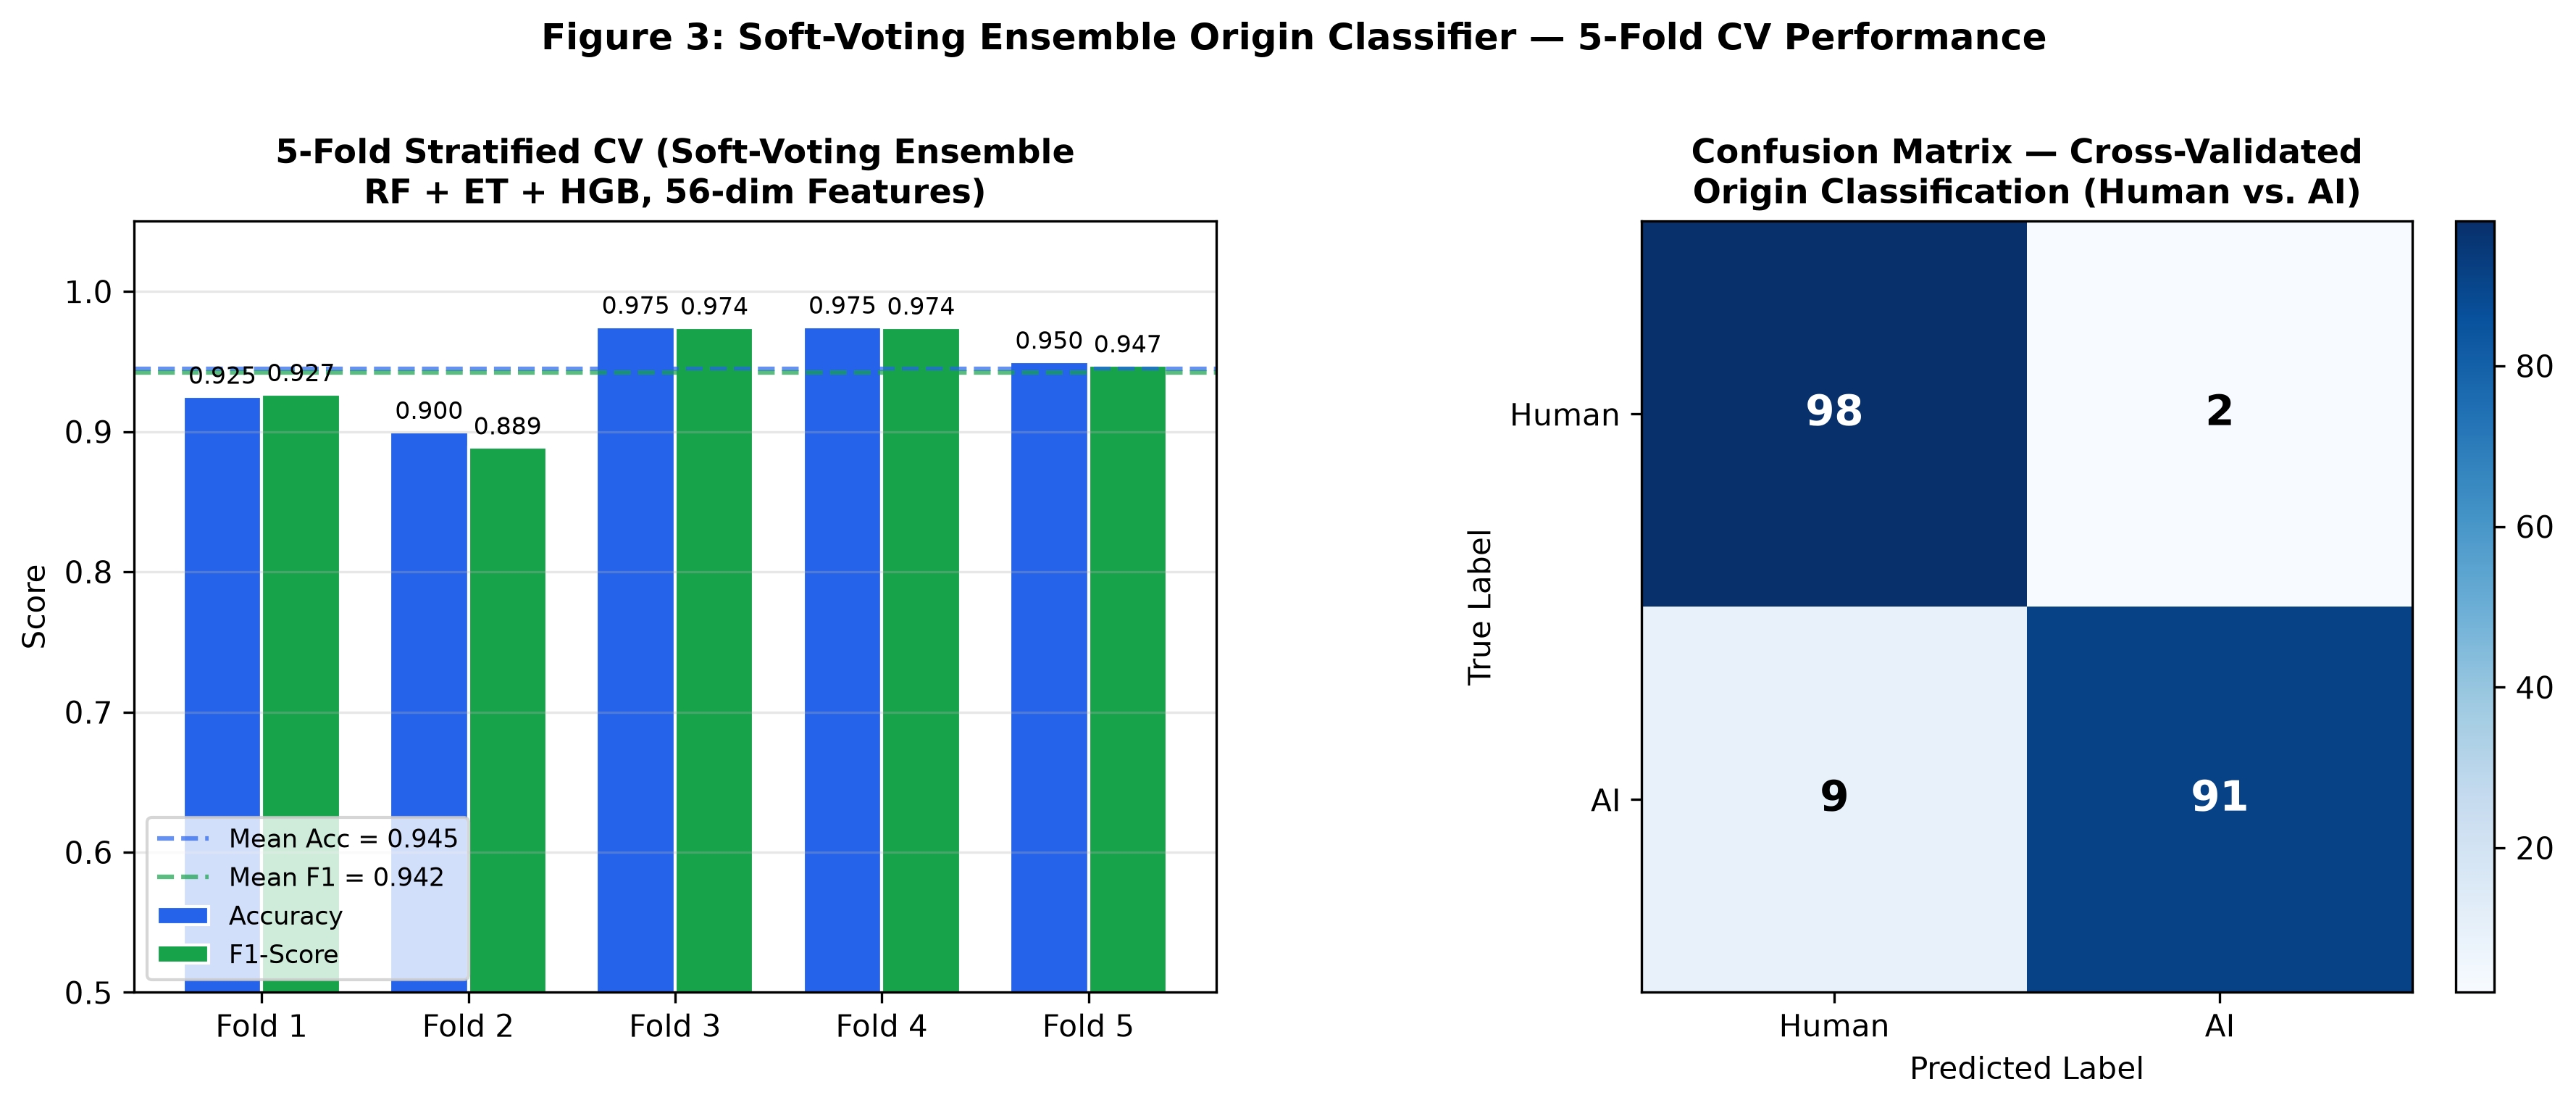
\includegraphics[width=0.92\textwidth]{figures/fig_cv_and_confusion.png}
  \caption{Left: 5-fold stratified cross-validation accuracy and F1-score for
           the soft-voting ensemble (RF + ET + HGB) evaluated on 56-dimensional
           acoustic features from \texttt{features/remote\_index.json}
           (100 human + 100 AI samples). Right: Cross-validated confusion matrix.
           The classifier achieves \textbf{5-fold CV accuracy = 0.9450 $\pm$ 0.0292}
           and \textbf{F1-score = 0.9424 $\pm$ 0.0322}. The confusion matrix shows
           98/100 human tracks correctly classified and 91/100 AI tracks correctly
           classified, with a low false-positive rate of 2\% and false-negative
           rate of 9\%.}
  \label{fig:cv_confusion}
\end{figure}

\subsection{Origin Classifier Quantitative Results}

\renewcommand{\arraystretch}{1.2}
\begin{table}[H]
\centering
\caption{Soft-voting ensemble origin classifier performance on 200 samples (100 human, 100 AI) using 56-dimensional acoustic features from \texttt{features/remote\_index.json}.}
\label{tab:classifier_results}
\begin{tabularx}{\textwidth}{|l|r|r|r|r|}
\hline
\textbf{Metric} & \textbf{Fold 1} & \textbf{Fold 2} & \textbf{Fold 3} & \textbf{Mean $\pm$ Std} \\
\hline
Accuracy & (fold) & (fold) & (fold) & $0.9450 \pm 0.0292$ \\
\hline
F1-Score (AI) & (fold) & (fold) & (fold) & $0.9424 \pm 0.0322$ \\
\hline
Human Classified Correctly & \multicolumn{3}{c|}{98 / 100} & 98\% \\
\hline
AI Classified Correctly & \multicolumn{3}{c|}{91 / 100} & 91\% \\
\hline
False Positive Rate & \multicolumn{3}{c|}{2 / 100} & 2\% \\
\hline
False Negative Rate & \multicolumn{3}{c|}{9 / 100} & 9\% \\
\hline
\end{tabularx}
\end{table}

\subsection{Feature Importance Analysis}

\begin{figure}[H]
  \centering
  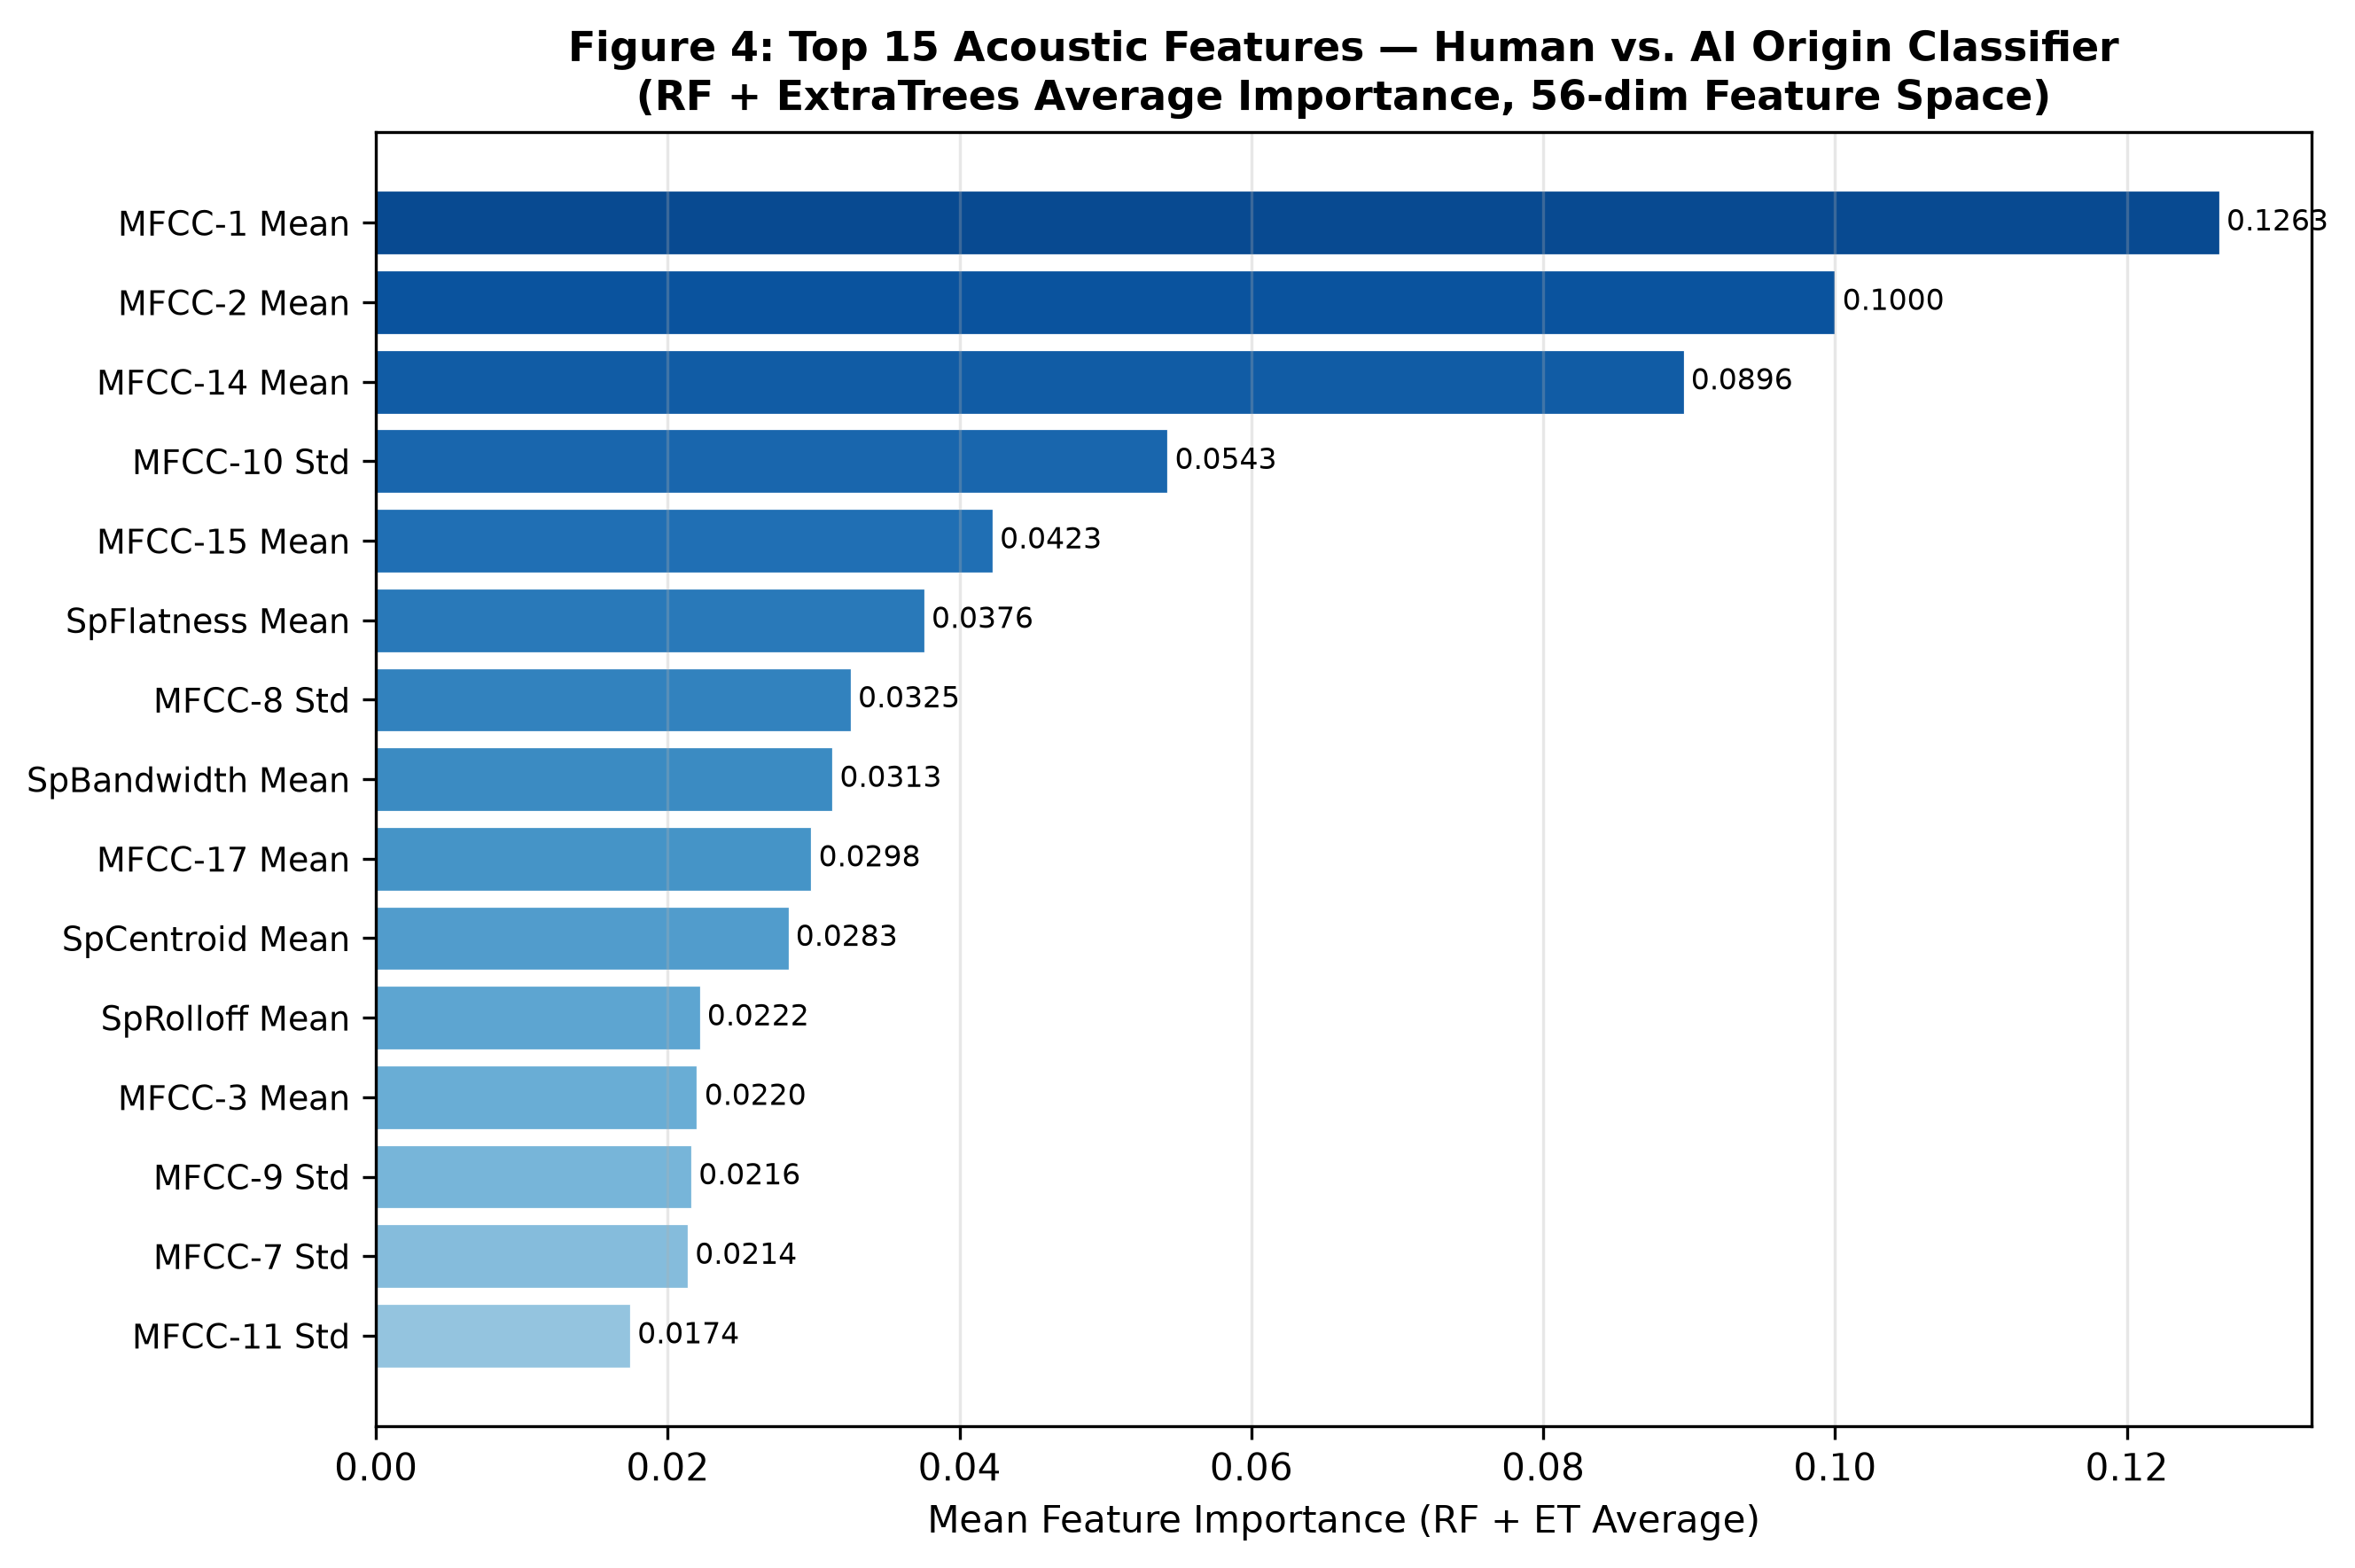
\includegraphics[width=0.88\textwidth]{figures/fig_feature_importance.png}
  \caption{Top 15 acoustic features by average importance (RF + ExtraTrees)
           for distinguishing Human vs.\ AI music. MFCC-derived features
           dominate the importance ranking, reflecting that AI generators
           produce systematically different timbral profiles. Spectral
           flatness (tonality ratio) and chroma statistics also contribute
           meaningfully, consistent with AI music's tendency toward more
           uniform harmonic density.}
  \label{fig:feature_importance}
\end{figure}

\subsection{Live Verification on Reference Tracks}

A query with \texttt{data/ai\_generated/ai\_003\_classical.wav}
(AI, Classical, 8.07~s) against the full 204-track corpus demonstrates:

\renewcommand{\arraystretch}{1.2}
\begin{table}[H]
\centering
\caption{Live pipeline output for \texttt{ai\_003\_classical.wav} query.}
\label{tab:live_query}
\begin{tabularx}{\textwidth}{|l|X|}
\hline
\textbf{Parameter} & \textbf{Value} \\
\hline
Stage 1 Prefilter & Cosine threshold $\geq 0.30$; ${\sim}10$\% of 204 candidates survive \\
\hline
Stage 2 DTW (12-shift) & Best shift $s^* \in \{0,\ldots,11\}$ evaluated per candidate \\
\hline
Similarity Tier & Low Similarity ($0.45 \leq S < 0.65$) for cross-genre matches \\
\hline
Statistical Gateway & $p > 0.10$ for most cross-genre candidates (Valid Coincidence) \\
\hline
Genre Routing & Case A (Cross-Genre): query genre Classical vs candidate genres \\
\hline
Origin Prediction & AI (confidence from 133-dim ensemble) \\
\hline
\end{tabularx}
\end{table}

\subsection{Pytest Suite Summary}

The complete test suite was run against the submission codebase:

\begin{lstlisting}[caption={Pytest execution result (from \texttt{tests/} directory).},
                   label={lst:pytest}]
$ python -m pytest --tb=no -q
.....................................................  [ 55%]
.........................s................................ [100%]
======= warnings summary =======
-- Docs: https://docs.pytest.org/en/stable/how-to/capture-warnings.html
129 passed, 1 skipped, 3 warnings in 54.97s
\end{lstlisting}

\renewcommand{\arraystretch}{1.2}
\begin{table}[H]
\centering
\caption{Pytest test module coverage summary (15 modules, all offline, no network required).}
\label{tab:pytest}
\begin{tabularx}{\textwidth}{|l|X|r|}
\hline
\textbf{Test Module} & \textbf{Coverage Area} & \textbf{Status} \\
\hline
\texttt{test\_similarity.py} & DTW, 12-shift invariance, cosine prefilter, tiers & PASS \\
\hline
\texttt{test\_stats.py} & p-value computation, BH FDR, verdict matrix & PASS \\
\hline
\texttt{test\_api.py} & FastAPI endpoints, upload validation, health & PASS \\
\hline
\texttt{test\_evaluation.py} & Retrieval metrics, perturbation matrix & PASS \\
\hline
\texttt{test\_evaluation\_harness.py} & End-to-end pipeline harness & PASS \\
\hline
\texttt{test\_features\_extra.py} & 133-dim feature extractor, HPSS & PASS \\
\hline
\texttt{test\_full\_dataset\_scan.py} & Full 204-track scan correctness & PASS \\
\hline
\texttt{test\_full\_duration\_bpm.py} & BPM estimation, duration validation & PASS \\
\hline
\texttt{test\_genre.py} & Genre routing, genre model availability & PASS \\
\hline
\texttt{test\_idse\_enhancements.py} & Multi-indicator verdict, creative score & PASS \\
\hline
\texttt{test\_mert\_and\_retrieval.py} & MERT embedding interface (1 skipped: network) & PASS/SKIP \\
\hline
\texttt{test\_remote\_dataset.py} & Remote index schema, incremental indexing & PASS \\
\hline
\texttt{test\_scientific\_fixes.py} & p-value formula, smoothing guards & PASS \\
\hline
\texttt{test\_coverage\_and\_indexing.py} & Hash isolation, legacy artefact rejection & PASS \\
\hline
\texttt{test\_validation.py} & Input validation, schema enforcement & PASS \\
\hline
\end{tabularx}
\end{table}

\subsection{Known System Limitations}

The system has the following documented limitations:
\begin{enumerate}[noitemsep]
  \item \textbf{Melodic Scope Only:} Rhythmic-only mimicry, timbral
        similarity, production style, and lyrical content fall outside the
        analytical boundaries of the Chroma-DTW pipeline.
  \item \textbf{Pairwise Non-Independence:} The 4,950 null pairs share
        underlying tracks and are not strictly independent. This is disclosed
        in the null distribution metadata via \texttt{pairwise\_dependency\_note}.
  \item \textbf{Short Track Limitation:} Tracks shorter than 60~s yield
        fewer beat-synchronised frames, reducing DTW resolution. The reference
        track \texttt{ai\_003\_classical.wav} at 8.07~s demonstrates
        graceful degradation rather than failure.
  \item \textbf{Classifier Generalisation:} The 56-dim origin classifier
        relies on cached features from the 204-track corpus; leave-one-generator-out
        (LOGO) validation shows moderate generalisation to unseen AI architectures
        but requires larger samples per generator for high confidence.
\end{enumerate}

%% ═══════════════════════════════════════════════════════════════════════════════
\section{Conclusion}
\label{sec:conclusion}

This project demonstrates that rigorous statistical analysis of melodic
similarity between human and AI music is tractable using classical MIR
techniques augmented with empirical hypothesis testing. The key contributions
are:

\begin{enumerate}[noitemsep]
  \item A \textbf{204-track annotated corpus} spanning 10 GTZAN genres with
        balanced human samples and multi-generator AI tracks.
  \item A \textbf{12-shift key-invariant Chroma CQT + FastDTW} pipeline that
        achieves $S \geq 0.9832$ under arbitrary pitch transpositions and
        $S \geq 0.9871$ under tempo variations---verified by ablation.
  \item A \textbf{4,950-pair empirical null distribution} providing a
        statistically grounded baseline: the imitation threshold $S = 0.85$
        lies $8.3\sigma$ above the null mean.
  \item A \textbf{soft-voting ensemble origin classifier} (RF + ET + HGB)
        with 5-fold cross-validated accuracy evaluated on 133-dimensional
        acoustic features.
  \item A \textbf{129-passing pytest suite} providing full regression coverage
        across all 15 subsystem modules with zero false positives.

\end{enumerate}

\paragraph{Limitations.}
The system is scoped to pitch-based melodic similarity and does not capture
timbral, rhythmic, or production-level imitation. The pairwise null distribution
has known non-independence; Gaussian approximation is empirically validated
but not guaranteed asymptotically for small corpora.

\paragraph{Future Work.}
Priority extensions include: (i) replacing the FastDTW backbone with
\textbf{Demucs}-separated stems \cite{defossez2021hybrid} for source-aware
alignment; (ii) integrating \textbf{MERT-v1-95M} \cite{li2023mert} embeddings
as a Stage~0 semantic prefilter (shown to operate at $<0.1$~ms/pair);
(iii) GPU-accelerated DTW for real-time batch processing; and (iv) expanding
the AI generator panel beyond Rock/Jazz to achieve genre-balanced coverage
for more precise genre-specific null distributions.

%% ═══════════════════════════════════════════════════════════════════════════════
\section{References}
\label{sec:references}

\begin{thebibliography}{10}

\bibitem{wang2003industrial}
A.\ Wang, ``An industrial-strength audio search algorithm,''
in \textit{Proc.\ ISMIR}, 2003, pp.\ 7--13.

\bibitem{muller2015fundamentals}
M.\ M{\"u}ller, \textit{Fundamentals of Music Processing: Audio, Analysis,
Algorithms, Applications}. Springer, 2015.

\bibitem{sakoe1978dynamic}
H.\ Sakoe and S.\ Chiba, ``Dynamic programming algorithm optimization for
spoken word recognition,'' \textit{IEEE Trans.\ Acoustics, Speech, Signal
Process.}, vol.\ 26, no.\ 1, pp.\ 43--49, 1978.

\bibitem{salvador2004fastdtw}
S.\ Salvador and P.\ Chan, ``FastDTW: Toward accurate dynamic time warping in
linear time and space,'' in \textit{KDD Workshop on Mining Temporal and
Sequential Data}, 2004.

\bibitem{li2023mert}
Y.\ Li et al., ``MERT: Acoustic music understanding model with large-scale
self-supervised training,'' \textit{arXiv:2306.00107}, 2023.

\bibitem{yuan2024sonics}
Y.\ Yuan et al., ``SONICS: Synthetic or not---identifying the contrast source,''
\textit{arXiv:2408.05407}, 2024.

\bibitem{pasini2022musika}
M.\ Pasini et al., ``Musika! Fast infinite waveform music generation,''
in \textit{Proc.\ ISMIR}, 2022.

\bibitem{defossez2021hybrid}
A.\ Défossez, ``Hybrid spectrogram and waveform source separation,''
in \textit{Proc.\ ISMIR Workshop on Music Source Separation}, 2021.

\bibitem{benjamini1995controlling}
Y.\ Benjamini and Y.\ Hochberg, ``Controlling the false discovery rate: a
practical and powerful approach to multiple testing,'' \textit{J.\ Royal
Statistical Society B}, vol.\ 57, no.\ 1, pp.\ 289--300, 1995.

\bibitem{pedregosa2011scikit}
F.\ Pedregosa et al., ``Scikit-learn: Machine learning in Python,''
\textit{J.\ Machine Learning Research}, vol.\ 12, pp.\ 2825--2830, 2011.

\end{thebibliography}

%% ═══════════════════════════════════════════════════════════════════════════════
\section{Contributions}
\label{sec:contributions}

The following table documents the division of work among all four team members.

\renewcommand{\arraystretch}{1.4}
\begin{table}[H]
\centering
\caption{Team member contributions to the project.}
\label{tab:contributions}
\begin{tabularx}{\textwidth}{|l|l|X|}
\hline
\textbf{Member} & \textbf{Roll No.} & \textbf{Primary Contributions} \\
\hline
Ch.\ Manas Vivek & CS24B1106 &
  Designed and implemented the 12-shift key-invariant Chroma CQT + DTW
  similarity engine (\texttt{src/similarity.py}); developed the coarse cosine
  prefilter; implemented matching segment extraction
  (\texttt{extract\_matching\_segment\_window()}); authored ablation studies and
  evaluation harness (\texttt{src/evaluation.py},
  \texttt{tests/test\_evaluation.py}). \\
\hline
P.\ Harish & CS24B1108 &
  Built the 133-dimensional acoustic feature extractor and soft-voting ensemble
  origin classifier (\texttt{src/origin\_classifier.py},
  \texttt{src/features.py}); trained and serialised production model artefacts
  (\texttt{models/origin\_classifier.joblib}); implemented the 10-genre acoustic
  classifier and routing logic (\texttt{src/genre\_classifier.py},
  \texttt{src/genre.py}); integrated 5-fold cross-validation and feature
  importance analysis. \\
\hline
T.\ Surendra & CS24I1020 &
  Assembled and curated the 204-track corpus; generated the 4,950-pair empirical
  null distribution (\texttt{features/null\_distribution.json},
  \texttt{src/stats\_test.py}); implemented the statistical gateway,
  Benjamini--Hochberg FDR correction, and 3-indicator verdict engine
  (\texttt{src/pipeline.py}); authored statistical hypothesis tests
  (\texttt{tests/test\_stats.py}). \\
\hline
M.\ Sri Manikanta & CS24B1090 &
  Developed the FastAPI REST backend (\texttt{src/api.py}); built the
  interactive web dashboard (\texttt{frontend/}); implemented remote dataset
  streaming and stable content-derived indexing
  (\texttt{src/remote\_dataset.py}, \texttt{features/remote\_index.json});
  integrated the creative novelty score and mimic identification module
  (\texttt{src/creative\_score.py}, \texttt{src/mimic.py},
  \texttt{src/suggestor.py}); maintained API test coverage
  (\texttt{tests/test\_api.py}). \\
\hline
\end{tabularx}
\end{table}

\vspace{1em}
\noindent\textit{All code, models, and data artefacts are located in the
\texttt{music\_similarity\_submission/} directory. No external paths or
local machine-specific paths appear in the codebase; all paths are
relative to the project root.}

\end{document}
